\section{Organizing and Analyzing Factors that Promote Evolvability}

\begin{frame}{Proximate/Ultimate Thinking}
  \begin{figure}
    \centering
    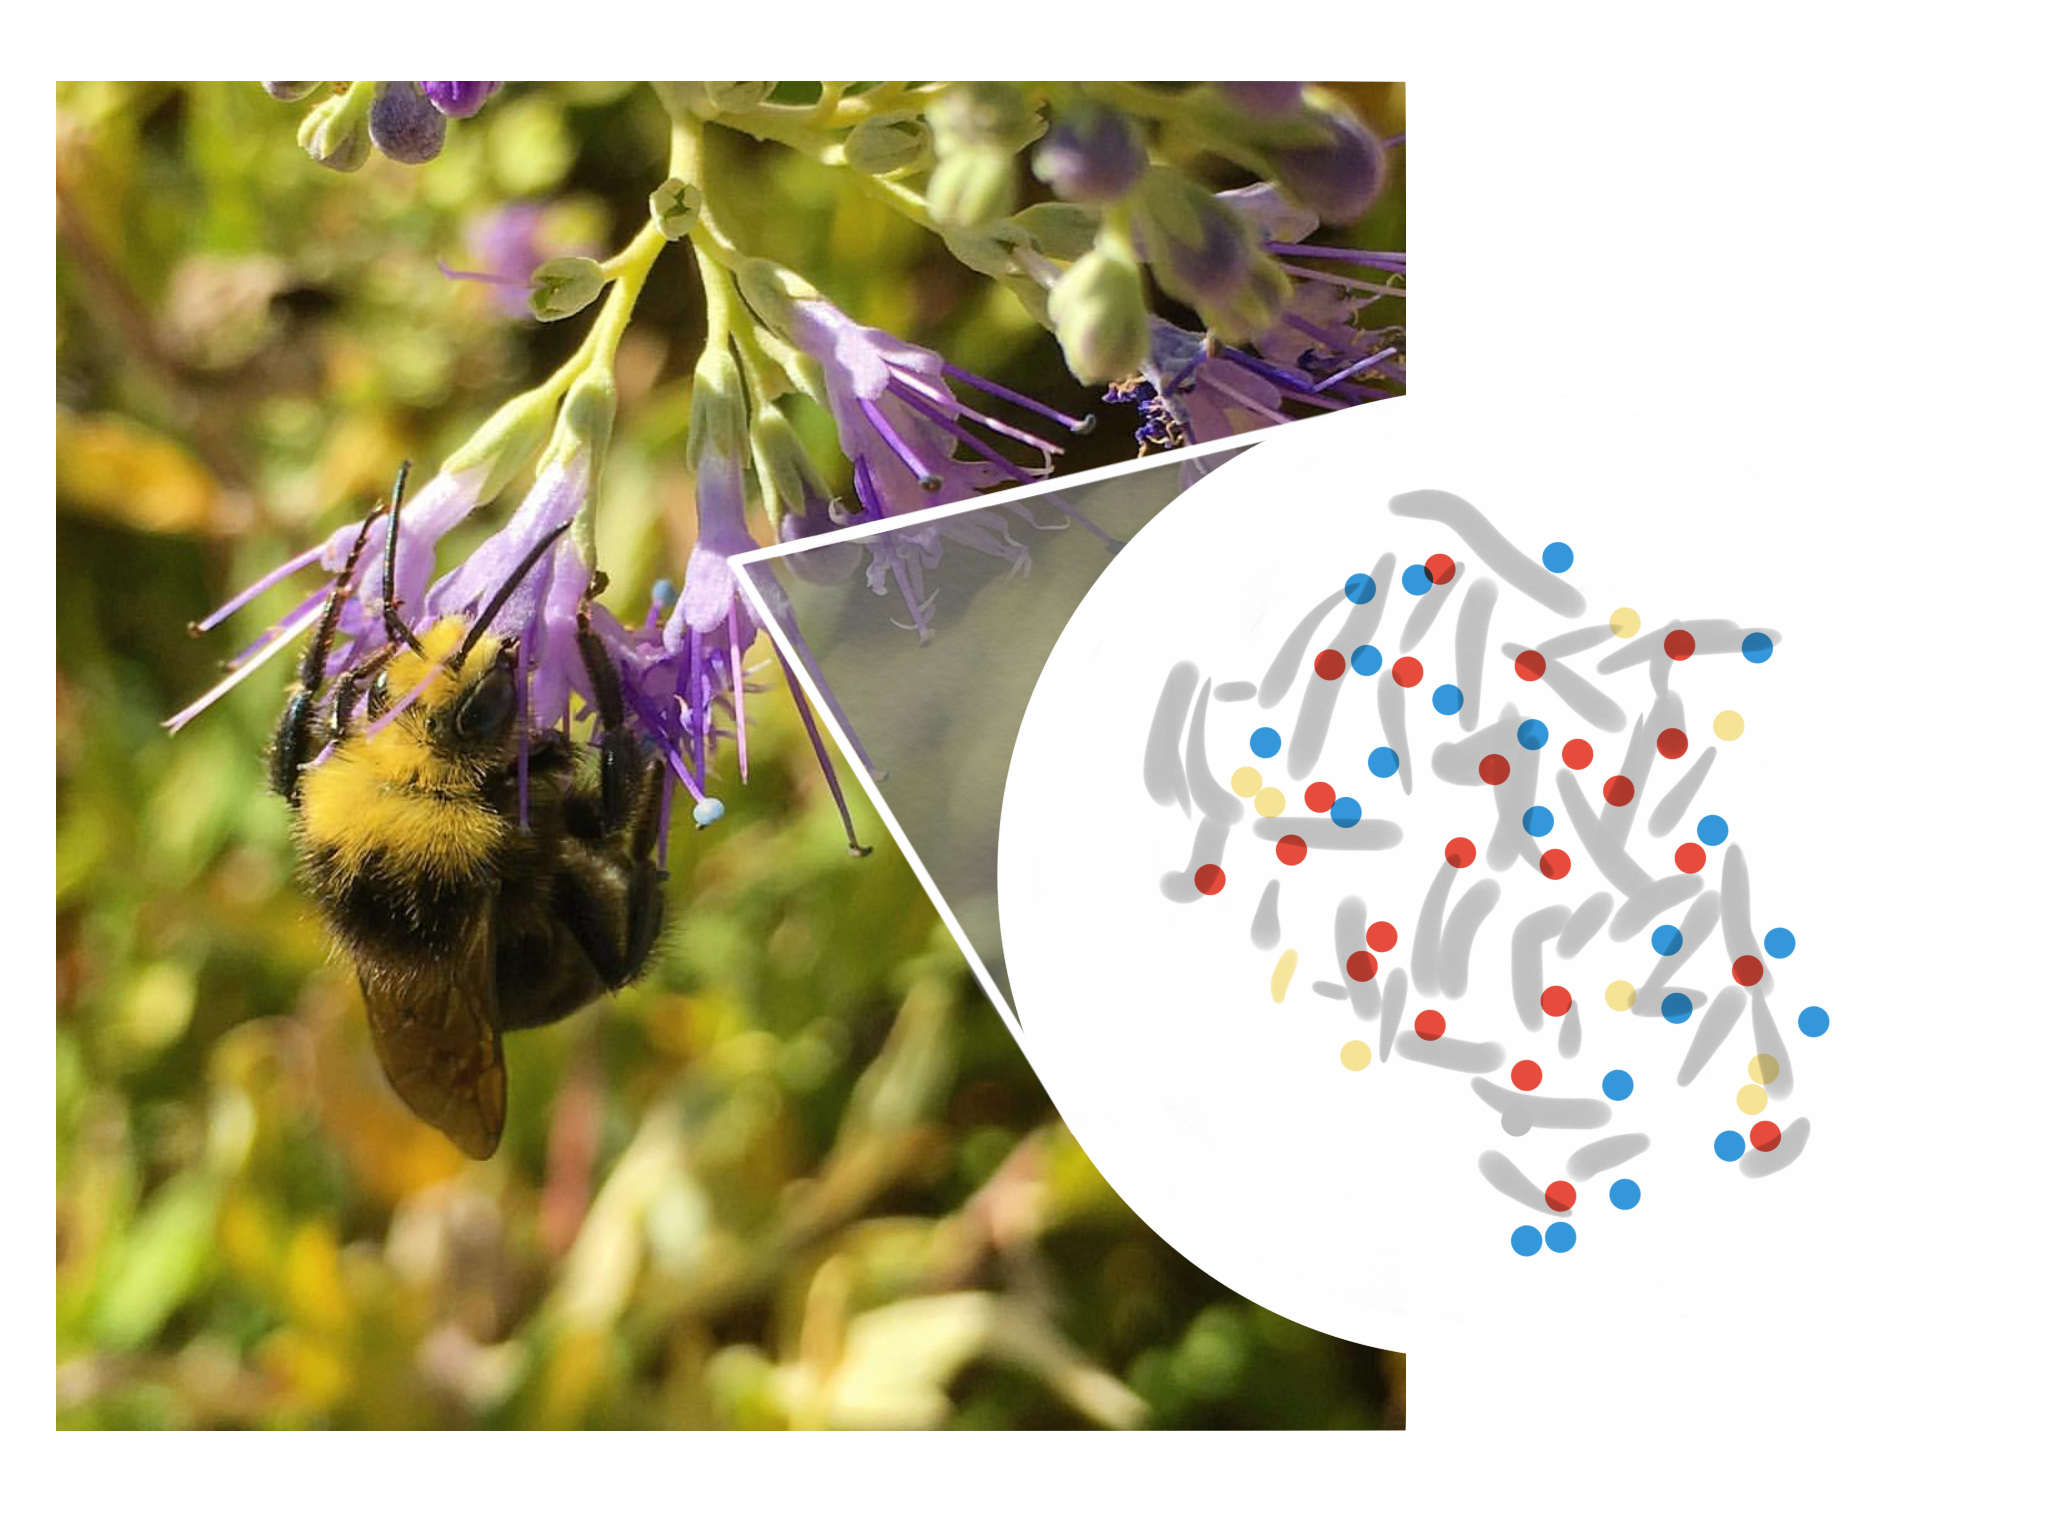
\includegraphics[width=0.8\textwidth]{img/proximate_ultimate}
 	\captionsetup{singlelinecheck=off,justification=raggedright}
  	\caption{Why is the flower purple? Proximate and ultimate explanations differ \cite{Wilson2007EvolutionLives}.}
    \label{fig:proximate_ultimate}
\end{figure}
\end{frame}

\begin{frame}{Proximate/Intermediate/Ultimate Organization}
\textbf{Proximate Causality}
\begin{itemize}
  \item describes specific organismal processes or structures 
\end{itemize}
\textbf{Intermediate Causality}
\begin{itemize}
  \item describes characteristics of an organism as a whole
\end{itemize}
\textbf{Ultimate Causality}
\begin{itemize}
  \item describes the relation between the individual and its environment
\end{itemize}
\end{frame}

\begin{frame}{Proximate/Intermediate/Ultimate Organization}
\begin{columns}[T,onlytextwidth]
\column{0.33\textwidth}
\textbf{Proximate Causality}
\begin{itemize}
  \item duplication and divergence
  \item developmental constraint
  \item hidden genetic variation
  \item exploratory growth
  \item weak linkage
  \item indirect encodings
\end{itemize}
\column{0.33\textwidth}
\textbf{Intermediate Causality}
\begin{itemize}
  \item modularity
  \item robustness
  \item canalization
  \item plasticity
  \item intraindividual degeneracy
  \item interindividual degeneracy
  \item regularity
\end{itemize}
\column{0.33\textwidth}
\textbf{Ultimate Causality}
\begin{itemize}
  \item temporally varying goals
  \item environmental influence on phenotype
  \item fitness degeneracy
\end{itemize}

\end{columns}
\end{frame}

\begin{frame}{Proximal Causality: Developmental Constraint}
  idea: the phenotype results from development, so developmental processes influence the phenotypic outcomes of mutation
    \begin{figure}
\begin{columns}
\begin{column}{0.7\textwidth}
  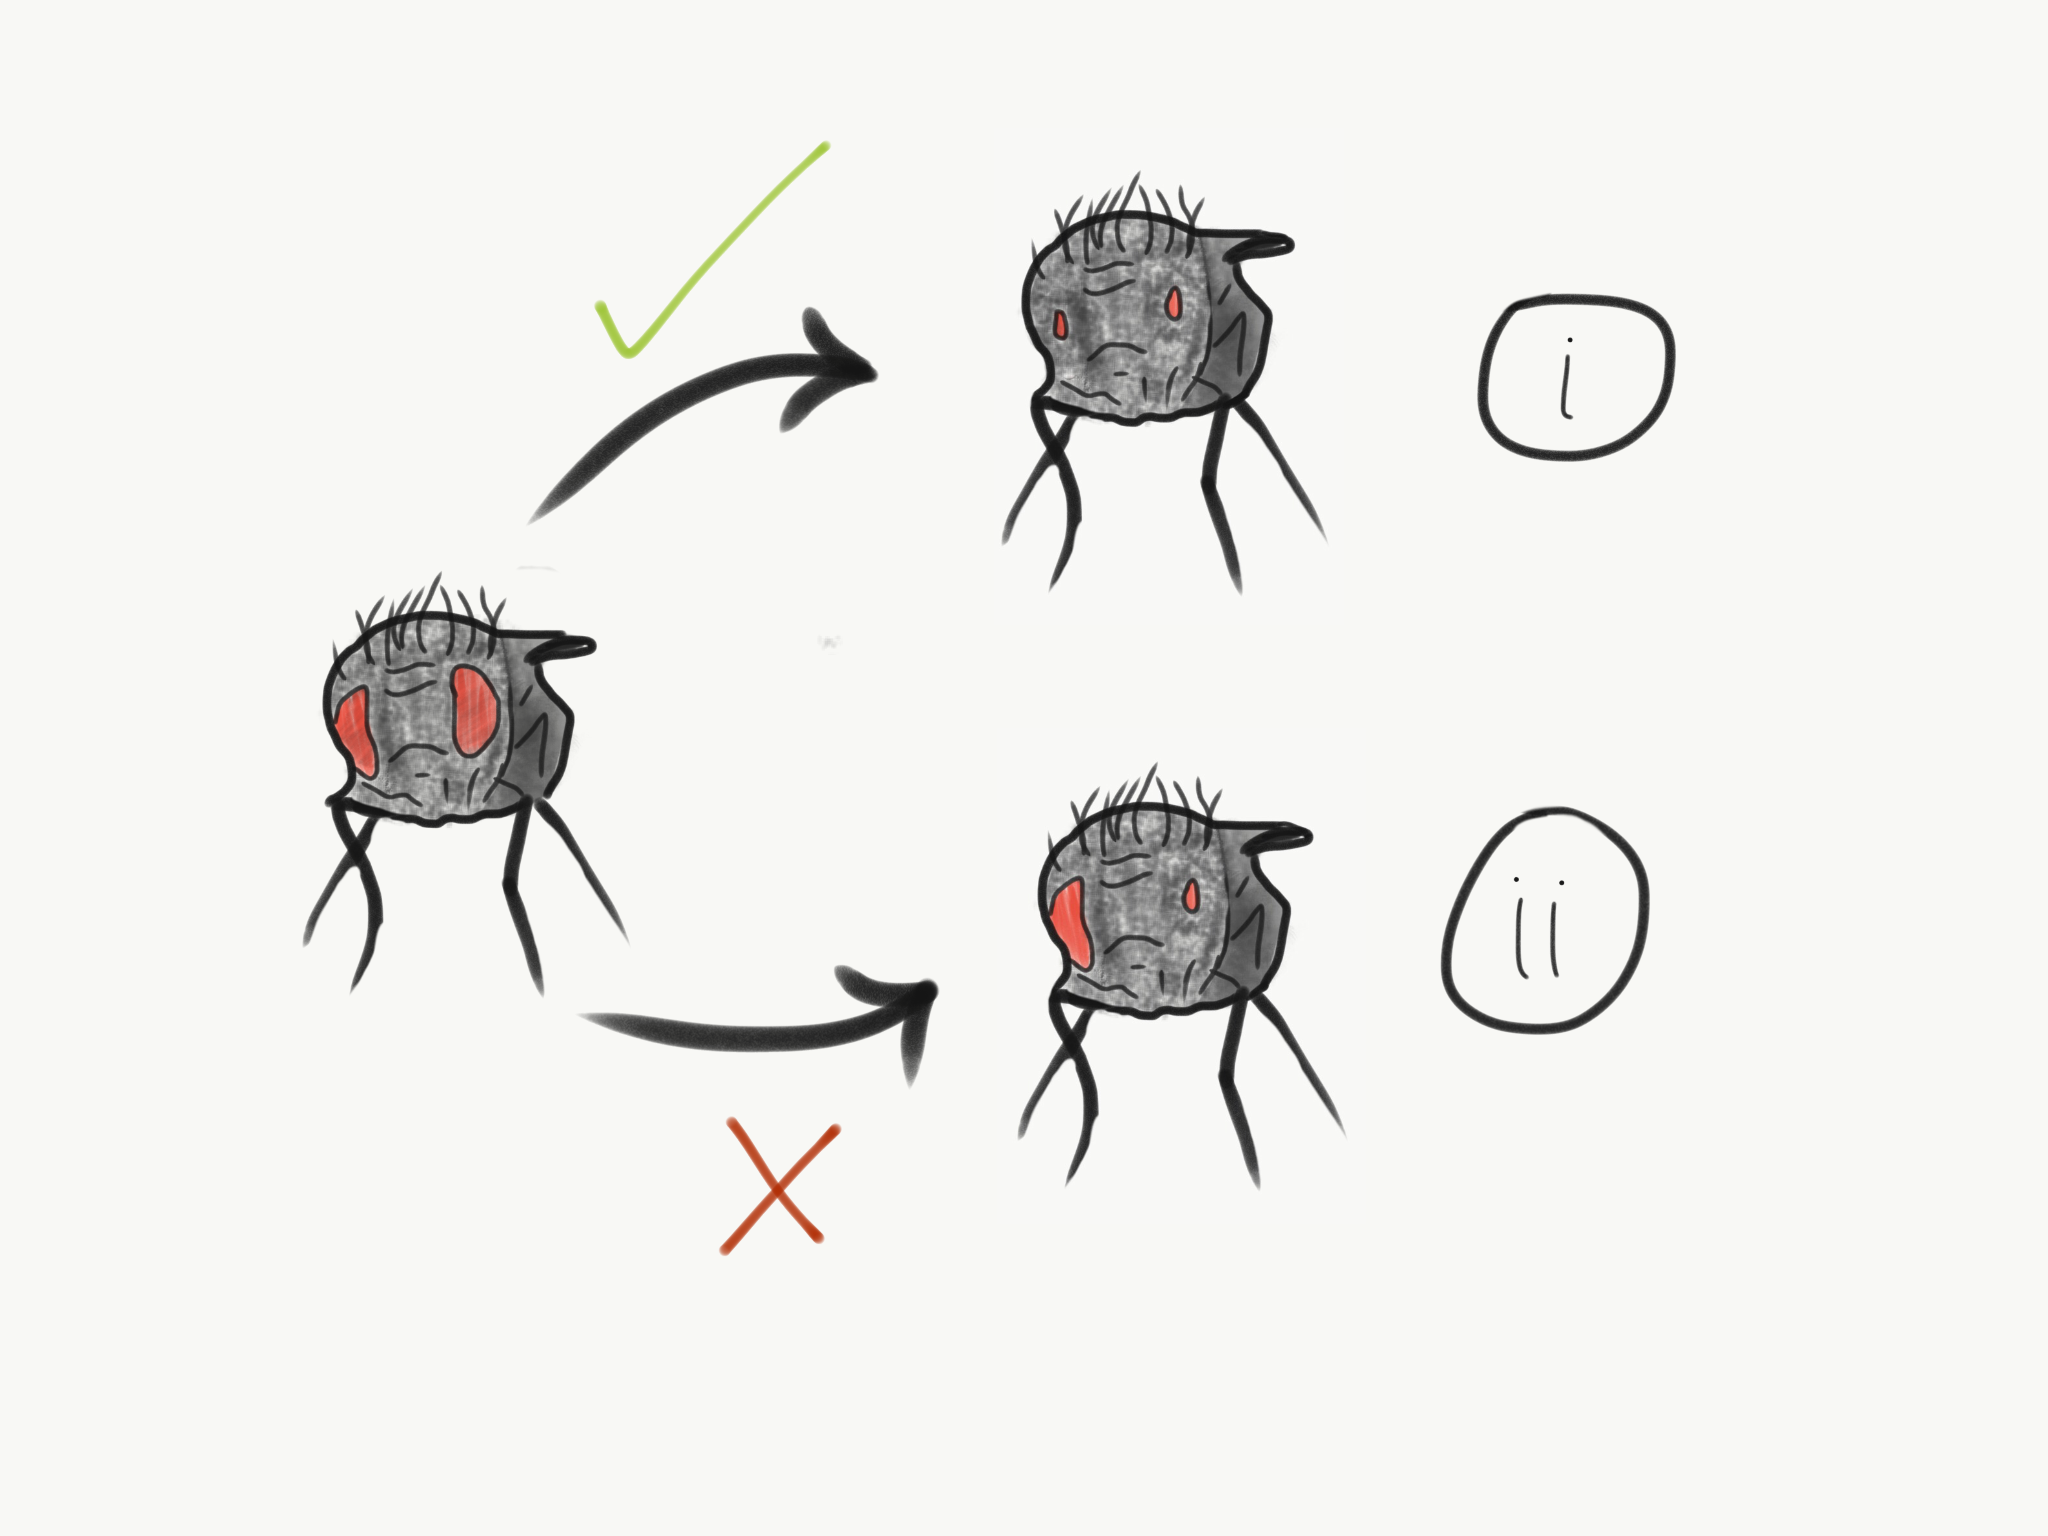
\includegraphics[width=\textwidth]{img/fly_canalization}
 \end{column}
 \begin{column}{0.3\textwidth}
  \caption{Illustration of Canalization Against Bilateral Asymmetry in \textit{Drosophilia melangoster} \cite{Tuinstra1990LackDevelopment}.}
  \label{fig:fly_canalization}
  \end{column}
  \end{columns}
\end{figure}
\end{frame}

\begin{frame}{Intermediate Causality: Intraindividual Degeneracy}
  idea: employing a diverse collection substructures that provide identical or near-identical functionality promote robustness through redundancy while providing many jumping off points for variation through repurposing or elaboration
  \begin{figure}
 \begin{columns}
 \begin{column}{0.6\textwidth}
 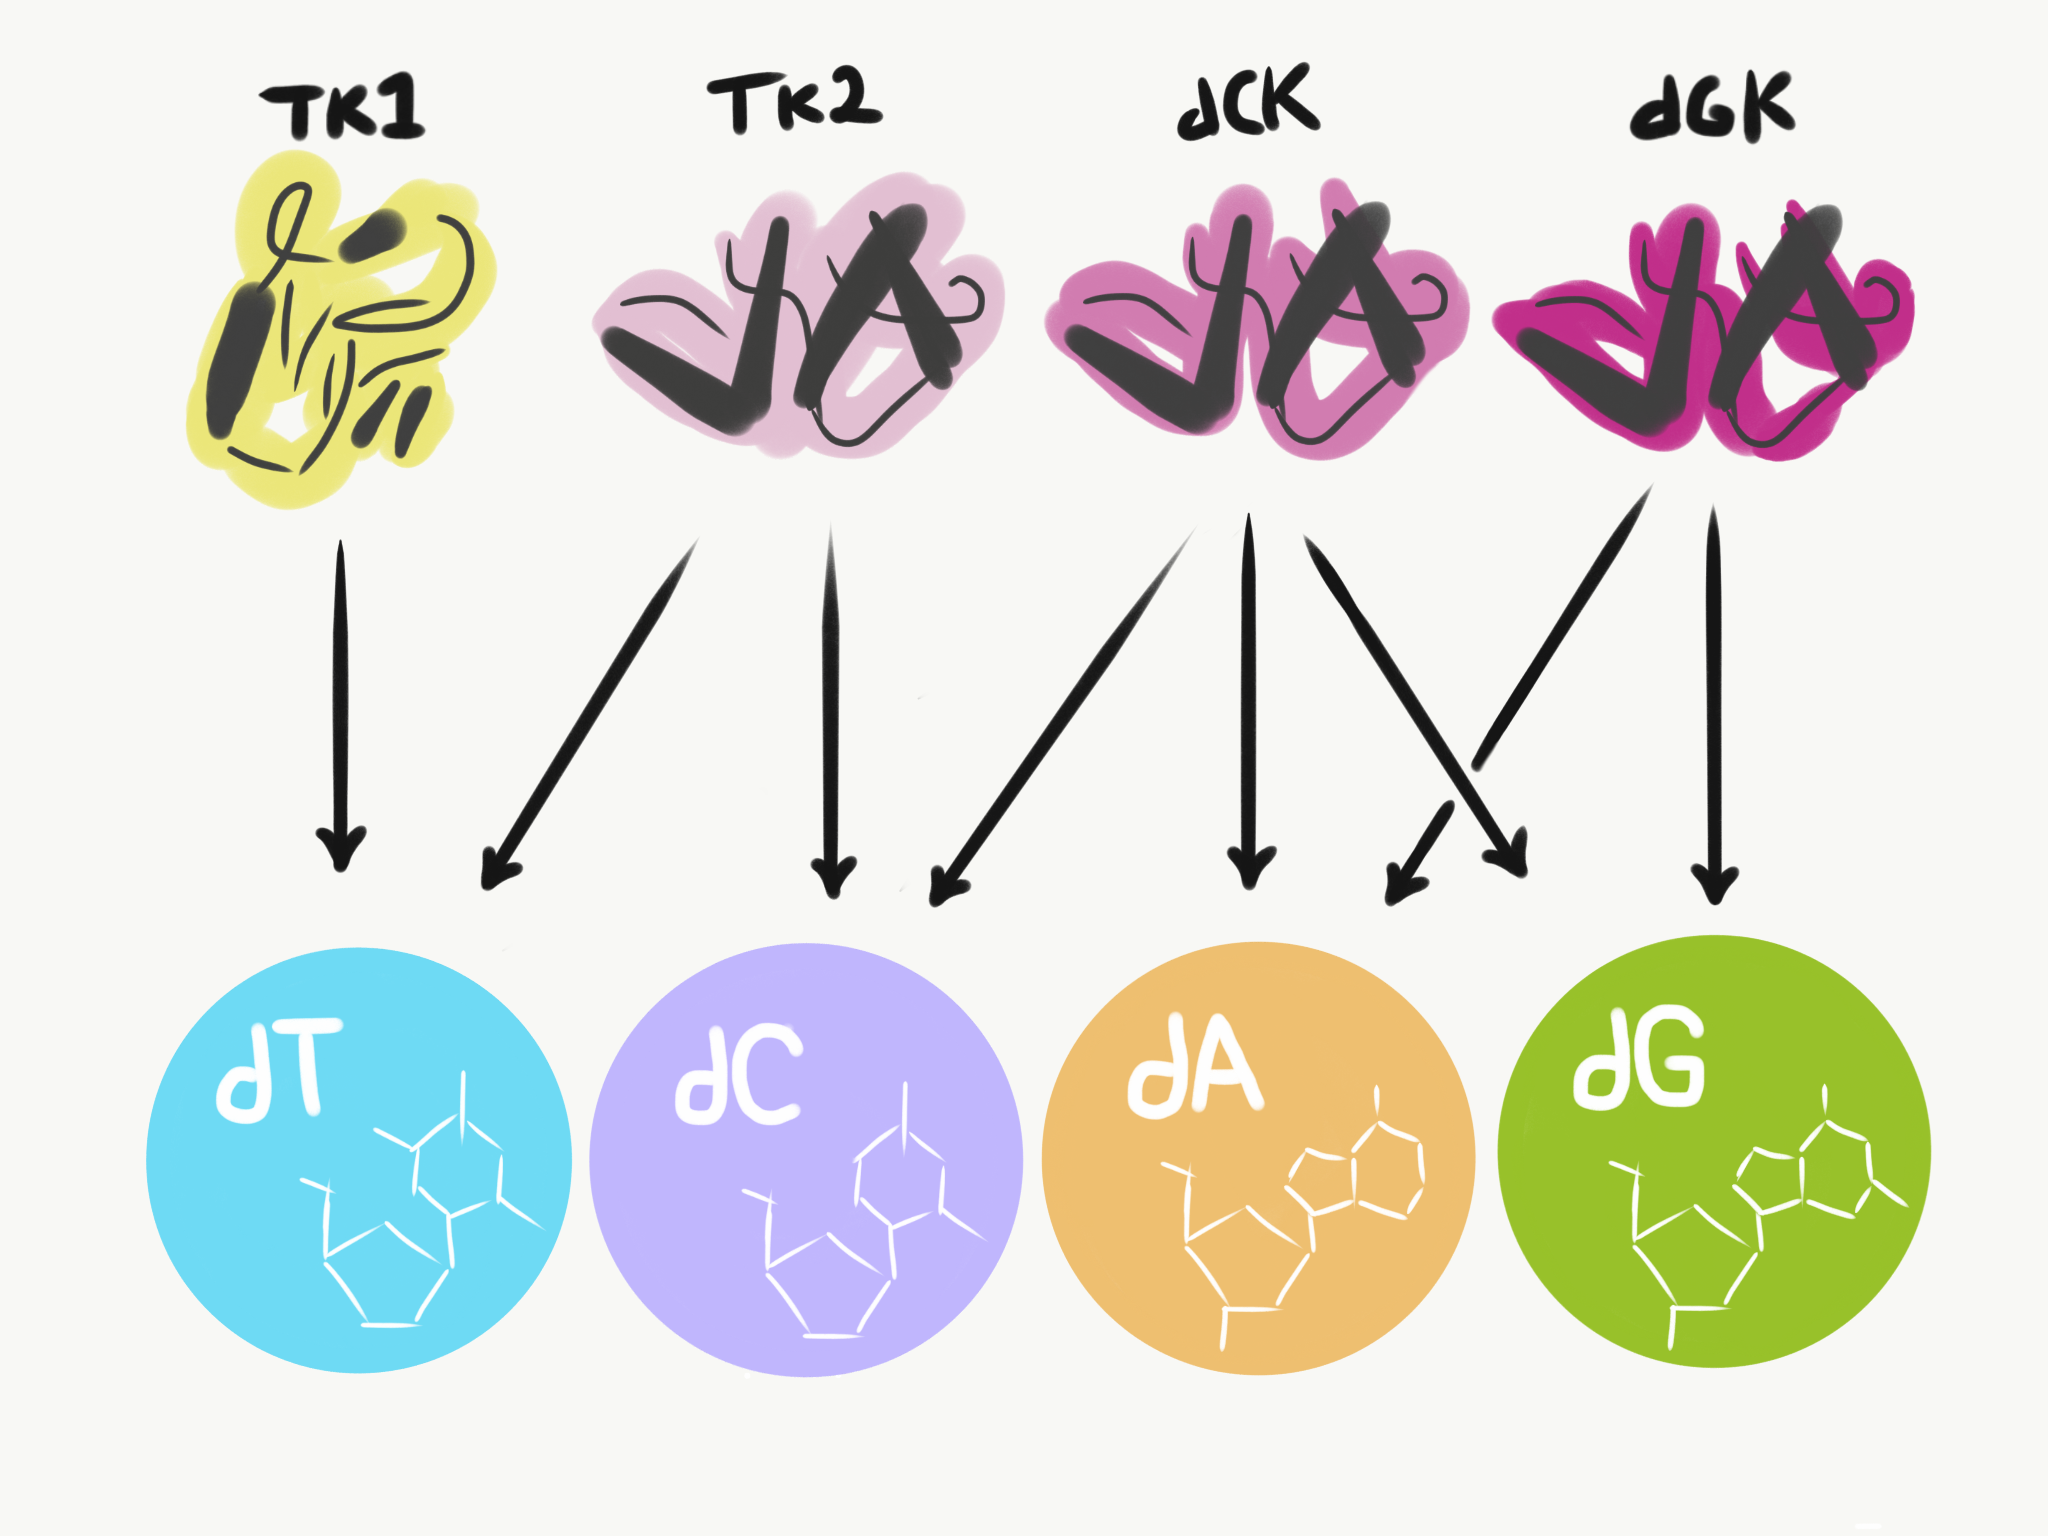
\includegraphics[width=\textwidth]{img/intraindividual_degeneracy}
 \end{column}
 \begin{column}{0.4\textwidth}
\captionsetup{singlelinecheck=off,justification=raggedright}
  	\caption{Mammalian deoxyribonucleoside kinases exhibit degeneracy \cite{Sandrini2005DeoxyribonucleosideReaction.}.}
    \label{fig:intraindividual_degeneracy}
    
\end{column}
\end{columns}
\end{figure}
\end{frame}

\begin{frame}{Ultimate Causality: Modularly Varying Fitness Function}
  idea: if evolution sets a moving target, organisms that produce variable offspring will be selected for 
  \begin{figure}

  \centering
  \begin{columns}[T,onlytextwidth]
\column{\textwidth}
\begin{minipage}[]{0.1\textwidth}
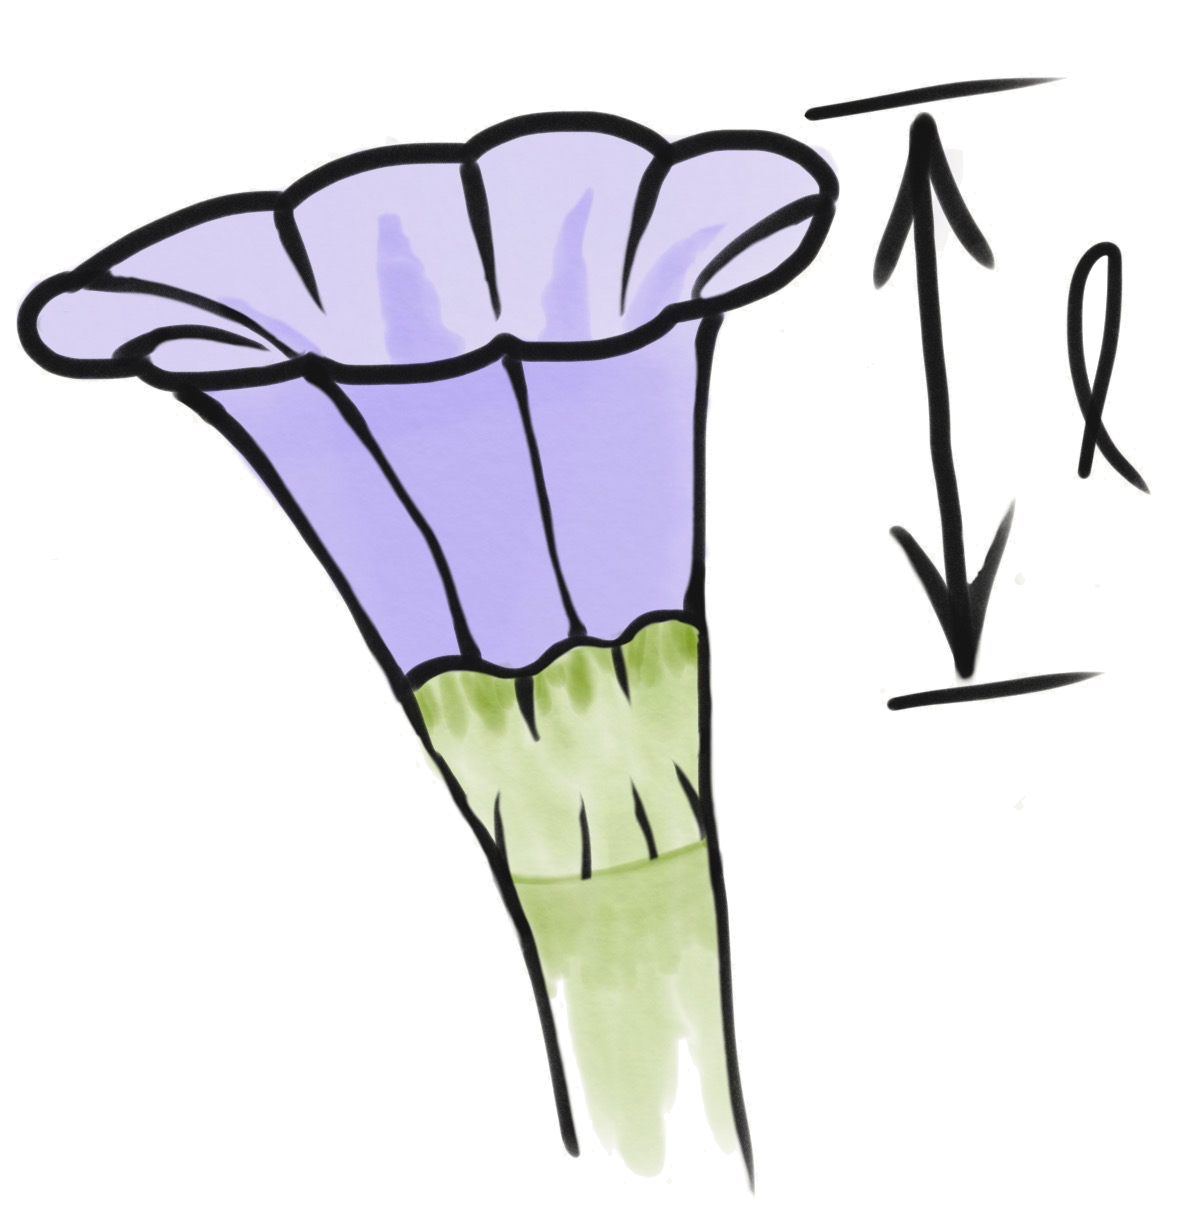
\includegraphics[width=\textwidth]{img/hbird_flower}
\end{minipage}%
\begin{minipage}[]{0.45\textwidth}
   \begin{subfigure}[b]{\textwidth}
    \centering
  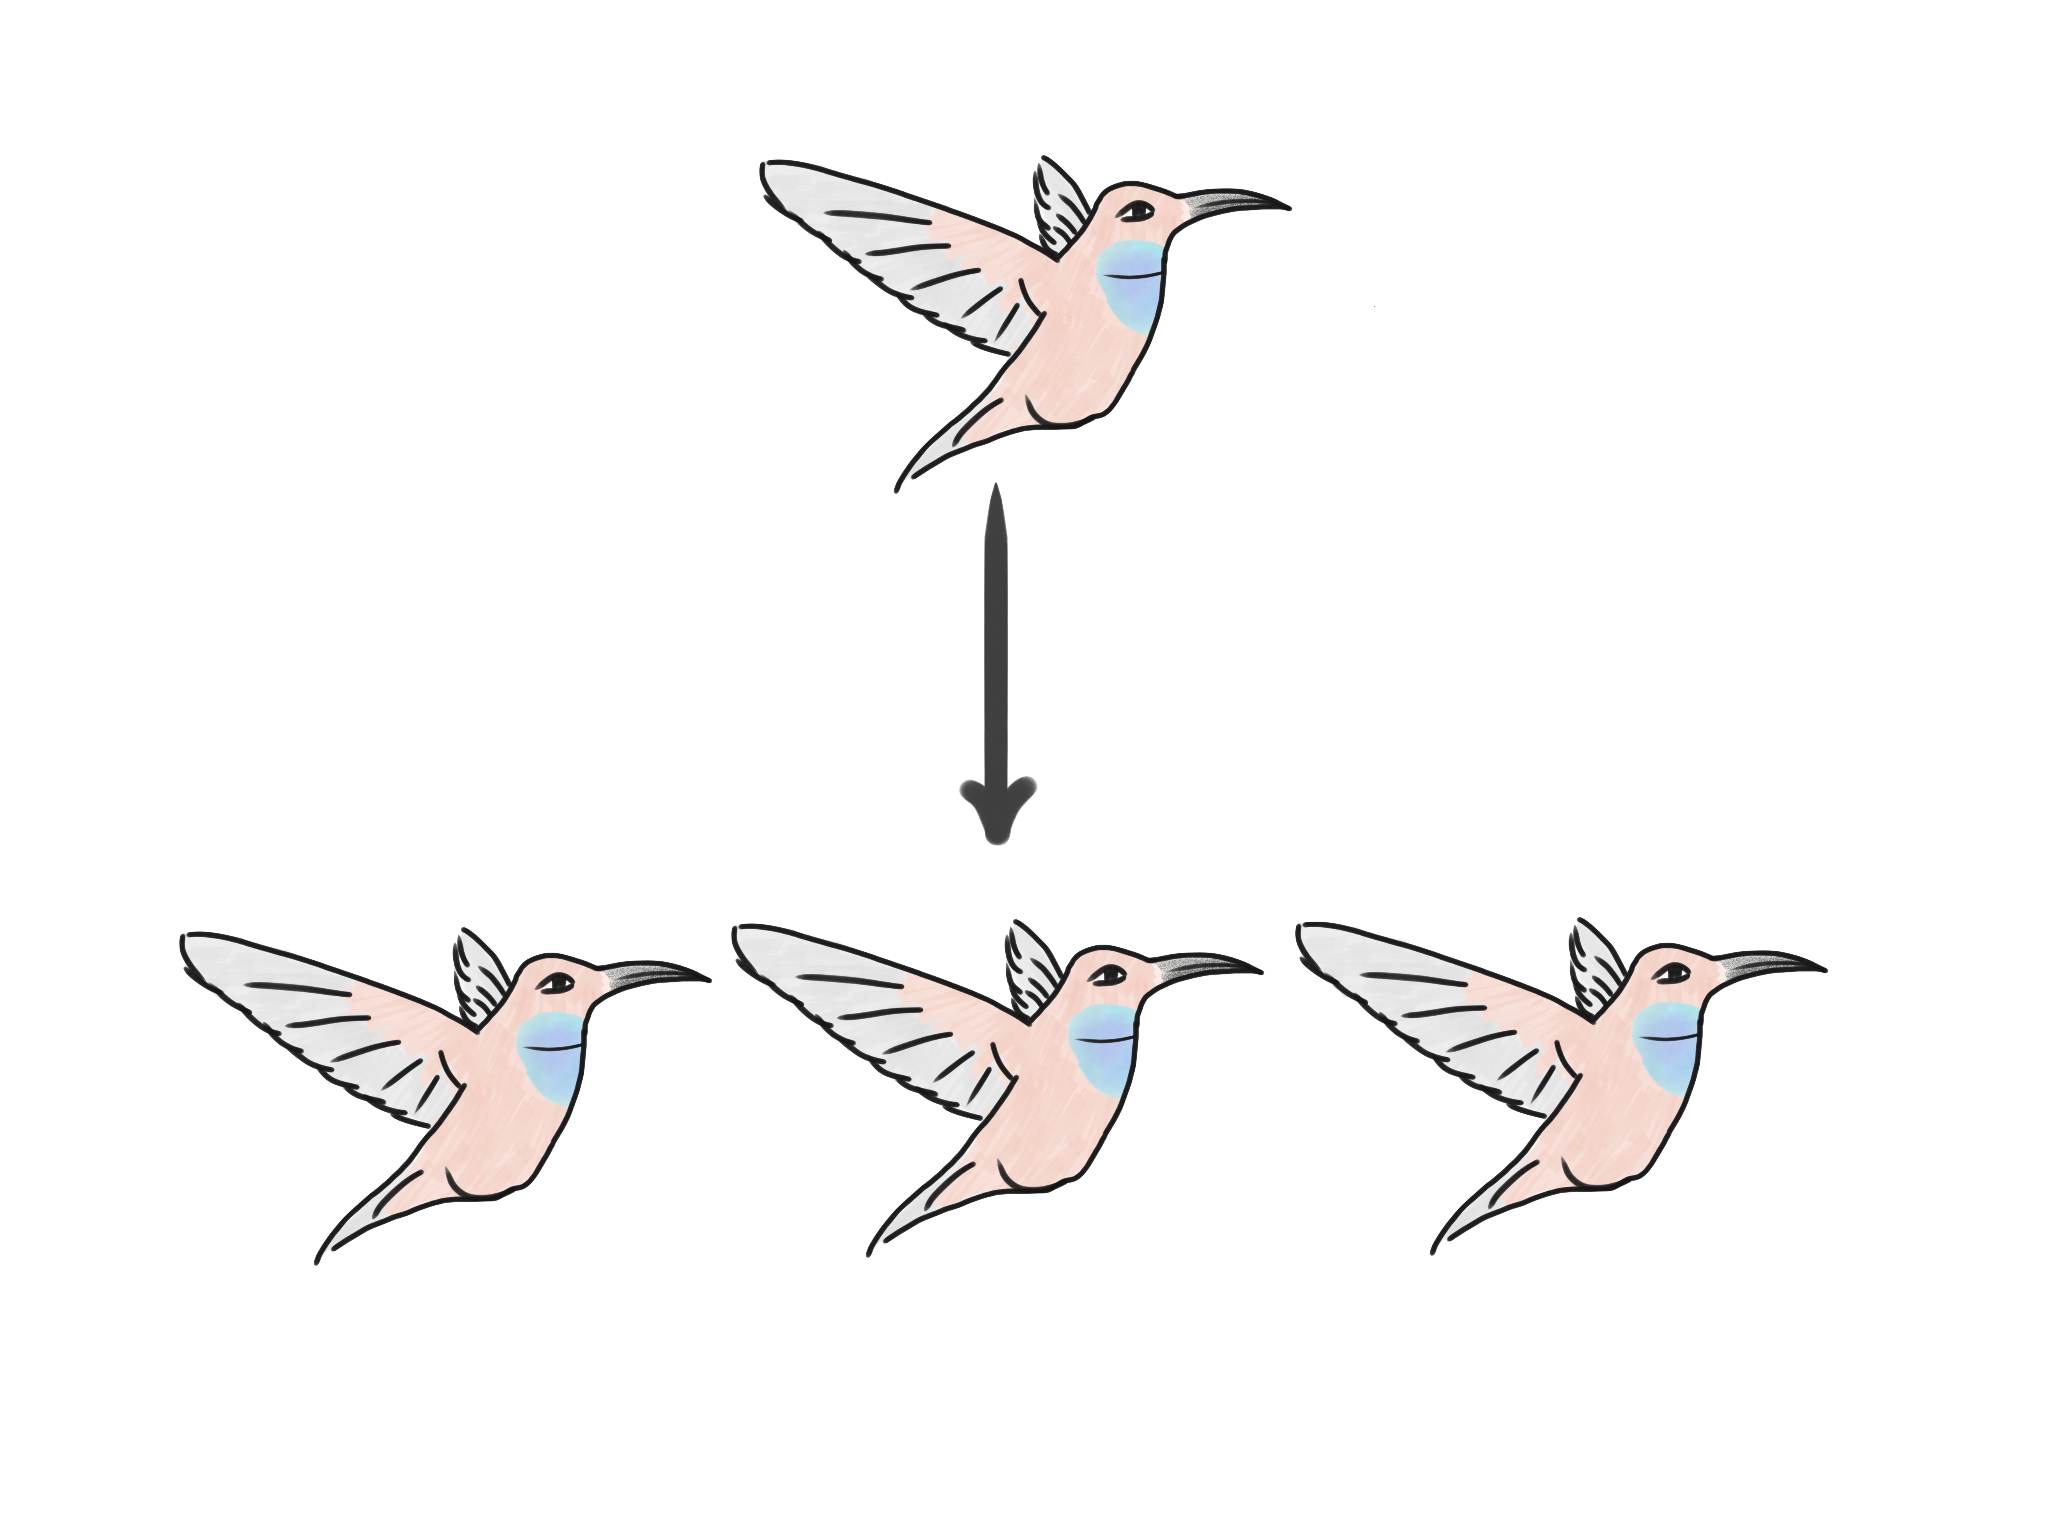
\includegraphics[width=\textwidth]{img/hbird_lowevol}
    \caption{low individual evolvability}
  \end{subfigure}%
\end{minipage}%
\begin{minipage}[]{0.45\textwidth}
\begin{subfigure}[b]{\textwidth}
    \centering
  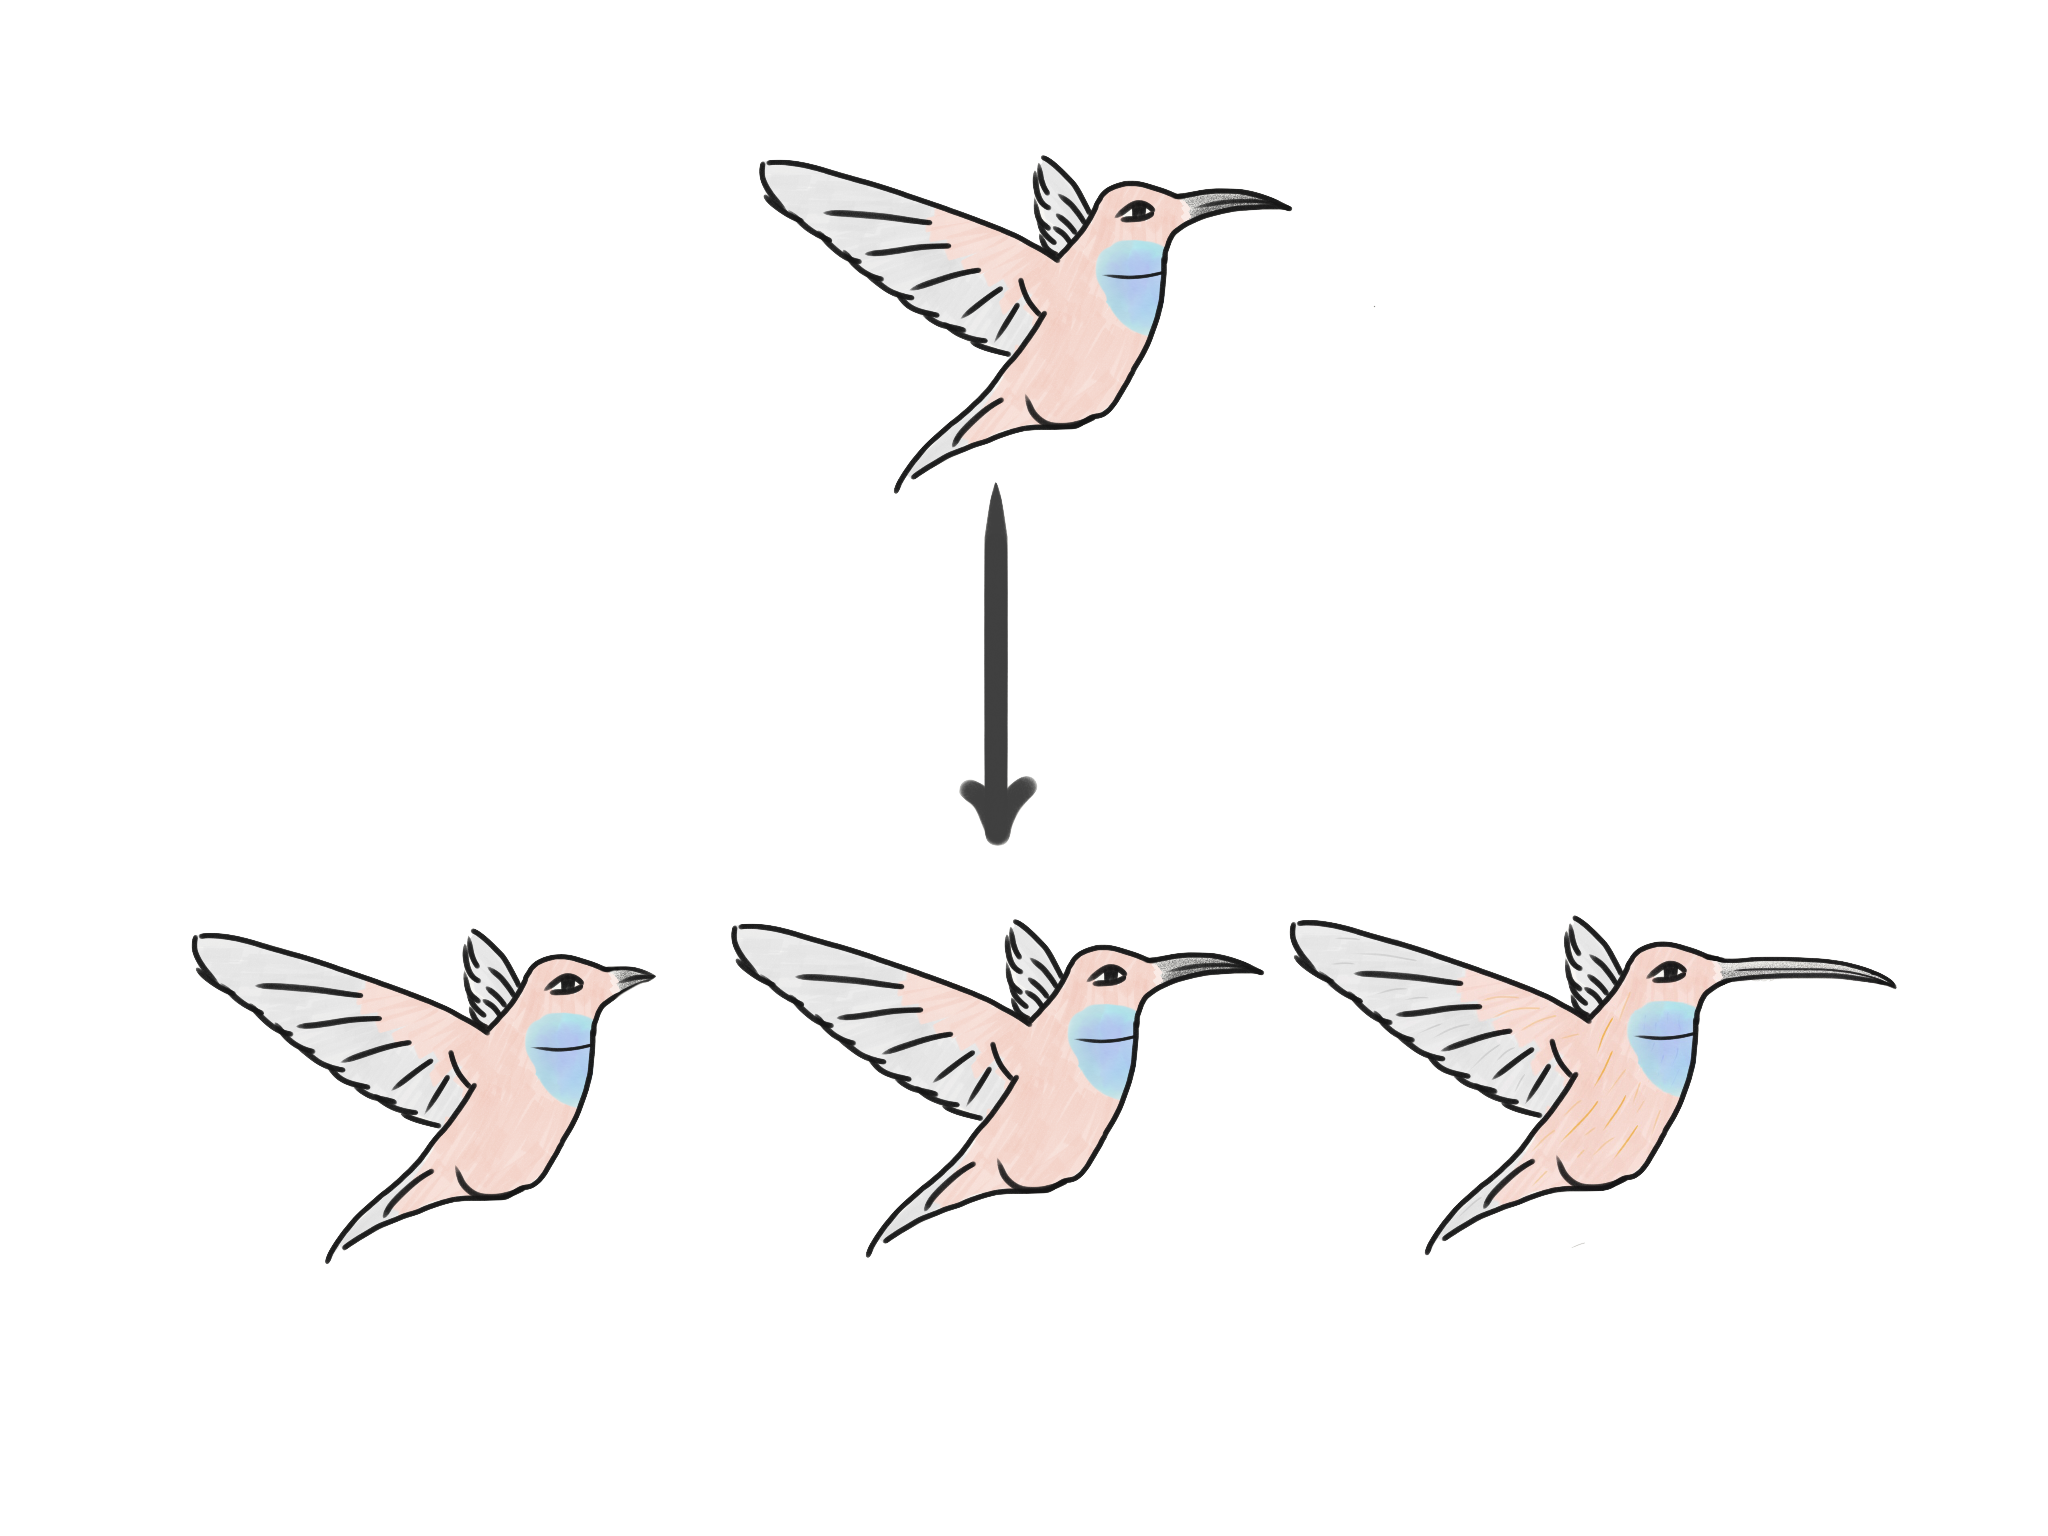
\includegraphics[width=\textwidth]{img/hbird_highevol}
    \caption{high individual evolvability}
  \end{subfigure}
\end{minipage}%
\end{columns}
 
\captionsetup{singlelinecheck=off,justification=raggedright}
  \caption{An hypothetical illustration of a modularly varying fitness function \cite{Kashtan2005SpontaneousMotifs}.}
  \label{fig:hummingbird_selection_pressure}
\end{figure}
\end{frame}

\begin{frame}{Analysis}
\alert{observations:}
\begin{itemize}
  \item proximal and intermediate causality relates to the genotype-phenotype mapping
  \item ultimate causality is related to interaction with the environment to determine fitness
\end{itemize}


\[\downarrow\]

\alert{paths forward:}
\begin{itemize}
\item taking a broader view of fitness and selection 
\item taking a more nuanced view of the developmental process
\end{itemize}
\end{frame}

% \begin{frame}{Analysis}
% \begin{itemize}
%   \item suggests two paths to getting evolvability:
%   \begin{itemize}
%     \item more nuanced artificial developmental process (genotype-phenotype mapping)
%     \item more open-ended selection
%   \end{itemize}
%   \item these paths are already well trod
% \end{itemize}
% \end{frame}